\begin{enumerate}
    \item Consider a random variable measuring the following quantities. In each case, state with reasons whether you think it is more appropriate to define the random variable as discrete or as continuous.
    \begin{enumerate}
        \item A person's height: Discrete. It is possible to measuring a person's height continuously, however, a person's height continuous changes, and hence measurements with units smaller than year quickly becomes meaningless.
        \item A student's course grade: Discrete. It is impossible grade a student's ability with precision.
        \item The thickness of a metal plate: Continuous. Measuring with continuity gives a better picture for how thickness changes overtime.
        \item The purity of a chemical solution: Continuous. Measuring with continuity gives a better picture for how the purity changes overtime.
        \item The type of personal computer a person owns: Discrete. There is a finite numbers of computer types.
        \item A person's age: Discrete. It is possible to measuring a person's age continuously, however, one's age continuously changes, and hence measurements with units smaller than year quickly becomes meaningless.
    \end{enumerate}
    \item A random variable $X$ takes values between 4 and 6 with a probability density function
    $$f(x)=\frac{1}{x\ln(1.50)}$$
    for $4\le x \le 6$ and $f(x)=0$ elsewhere.
    \begin{enumerate}
        \item Make a sketch of the probability density function.
        \begin{center}
            \begin{tikzpicture}
            \pgfkeys{/pgf/number format/fixed}
            \begin{axis}[
				axis lines=left,
                xmin=3, xmax=7,
                ymin = 0, ymax = 1,
                width=8cm,height=5cm
                ]
            \addplot[red, very thick, domain=4:6]{1/(x*ln(1.5))};
            \end{axis}
            \end{tikzpicture}
        \end{center}
        \item Check that the total area under the probability density function is equal to 1.
        \begin{equation*}
            \int_{-\infty}^{\infty}{f(x) \,dx} = 
            \int_{4}^{6}{\frac{1}{x\ln(1.5)}\,dx} =
            \left.\frac{\ln(x)}{\ln(1.5)}\right|_{x=4}^{x=6} = 1
        \end{equation*}
        \item What is $P (4.5 \le X \le 5.5)$?
        \begin{equation*}
            \int_{4.5}^{5.5}{\frac{1}{x\ln(1.5)}\,dx}
            = \left.\frac{\ln(x)}{\ln(1.5)}\right|_{x=4.5}^{x=5.5} = \ln(5.5/4.5) / \ln(1.5) \approx 0.4949148310
        \end{equation*}
        \item Construct and sketch the cumulative distribution function.\\
        For $x<4, F(x) = 0$. For $x>6, F(x) = 1$.\\
        For $4 \le x \le 6$,
        $$F(x) = \int_{4}^{x}{\frac{1}{t\ln(1.5)}\,dt} = \left.\frac{\ln(t)}{\ln(1.5)}\right|_{t=4}^{t=x} = \frac{\ln(x)-\ln(4)}{\ln(1.5)}$$

        \begin{center}
            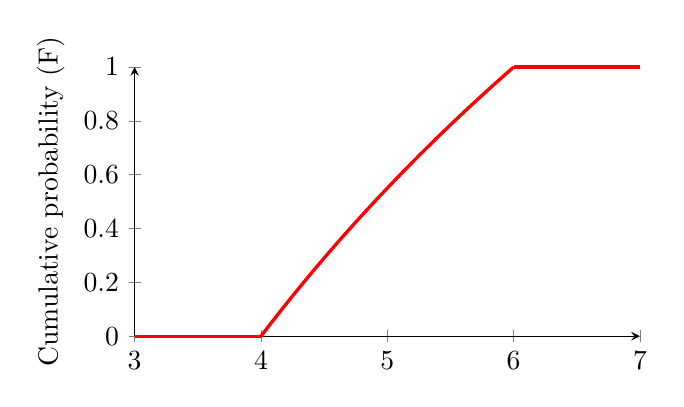
\begin{tikzpicture}
            \pgfkeys{/pgf/number format/fixed}
            \begin{axis}[
				axis lines=left,
                ylabel={Cumulative probability (F)},
                xmin=3, xmax=7,
                ymin = 0, ymax = 1, clip = false,
                width=8cm,height=5cm
                ]
            \addplot[red, very thick, domain=4:6]{(ln(x)-ln(4))/(ln(1.5))};
            \addplot[red, very thick, domain=3:4]{0};
            \addplot[red, very thick, domain=6:7]{1};
            \end{axis}
            \end{tikzpicture}
        \end{center}
        \item What is the expected value of this random variable?
        $$E(X) = \int_{4}^{6}{\frac{x}{x\ln(1.5)}\,dx} = \left.\frac{x}{\ln(1.5)}\right|_{x=4}^{x=6} = \frac{2}{\ln(1.5)} \approx 4.93260692475$$
        \item What is the median of this random variable?
        $$F(x) = 0.5 \Leftrightarrow \frac{\ln(x)-\ln(4)}{\ln(1.5)} = 0.5 \Leftrightarrow \ln(x)= 0.5\ln(1.5)+\ln(4) \Leftrightarrow x= 4\sqrt{1.5} = 2\sqrt{6}$$
        \item What is the variance and the standard deviation of this random variable?
        \begin{multline*}
            \n{Var}(X) = \int_{4}^{6}{\frac{x^2}{x\ln(1.5)}\,dx}-E(X)^2
            = \int_{4}^{6}{\frac{x}{\ln(1.5)}\,dx}-E(X)^2\\
            = \left.\frac{x^2}{2\ln(1.5)}\right|_{x=4}^{x=6} - E(X)^2
            = \frac{10}{\ln(1.5)} - E(X)^2 \approx 0.332423549644
        \end{multline*}
        $$\sigma = \sqrt{\n{Var}(X)} \approx 0.576561835057$$
    \end{enumerate}
    \item A random variable $X$ takes values between 0 and $\infty$ with a cumulative distribution function
    $$F(x)=A+Be^{-x}$$
    for $0 \le x < \infty$.
    \begin{enumerate}
        \item Find the values of $A$ and $B$ and sketch the cumulative distribution function.\\
        Since $1=\lim_{x \to \infty} F(x)$,$1 = \lim_{x \to \infty} A +Be^{-x} = A$.\\
        Hence $A = 1$.\\
        Since $X$ takes values between 0 and $\infty$, $F(0) = 0$ (X does not takes 0).\\
        Hence $F(0) = A + Be^{-x} = A + B = 0 \Rightarrow B = -1$.\\
        Therefore, $F(x) = 1 - e^{-x}$\\
        \begin{center}
            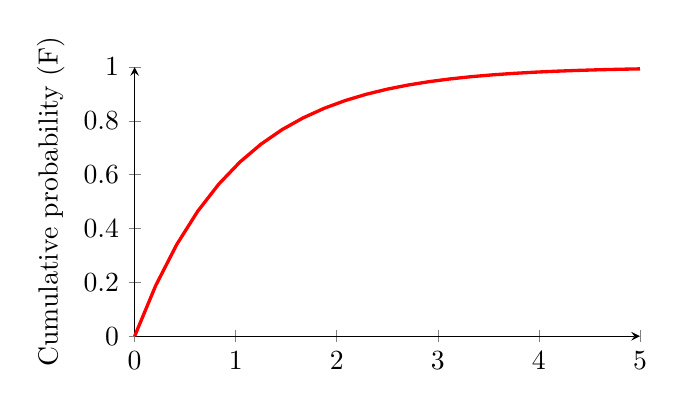
\begin{tikzpicture}
            \pgfkeys{/pgf/number format/fixed}
            \begin{axis}[
				axis lines=left,
                ylabel={Cumulative probability (F)},
                xmin=0, xmax=5,
                ymin = 0, ymax = 1,
                clip = false,
                width=8cm,height=5cm
                ]
            \addplot[red, very thick, domain=0:5]{1-e^(-x)};
            \end{axis}
            \end{tikzpicture}
        \end{center}

        \item What is $P (2 \le X \le 3)$?
        $$P (2 \le X \le 3) = F(3) - F(2) = e^{-2} - e^{-3} \approx 0.0855482149$$
        \item Construct and sketch the probability density function.\\
        For $0<x<\infty$,
        $$f(x) = \frac{d}{dx}\left(1 - e^{-x}\right) = e^{-x}$$
        
        \begin{center}
            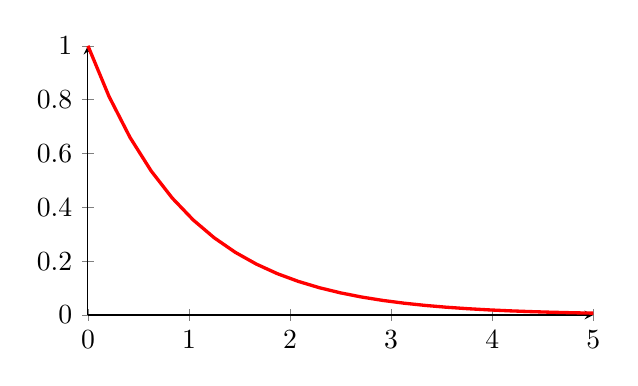
\begin{tikzpicture}
            \pgfkeys{/pgf/number format/fixed}
            \begin{axis}[
				axis lines=left,
                xmin=0, xmax=5,
                ymin = 0, ymax = 1,
                clip = false,
                width=8cm,height=5cm
                ]
            \addplot[red, very thick, domain=0:5]{e^(-x)};
            \end{axis}
            \end{tikzpicture}
        \end{center}
    \end{enumerate}
\end{enumerate}